\section{基于矩阵分解的单细胞 GRN 构建方法}
\label{sec:scgrnhunter}

\subsection{引言}

在第 \ref{sec:locpcacmi} 章和第 \ref{sec:d3grn} 章, 本文分别介绍了无向网络构建的 Loc-PCA-CMI 方法和有向网络构建的 D3GRN 方法, 
它们都是针对 DNA 微阵列测序技术下的基因表达数据集提出来的方法。
当使用的数据转向了单细胞 RNA-seq 数据集的时候, 
由于单细胞数据本身非常稀疏, 基因调控网络的构建也变得更加具有挑战性。
% 第 \ref{sec:rafclust} 章介绍了单细胞的细胞类型识别方法,
% 包括基于随机森林相似性学习的单细胞聚类方法 RafClust 
% 和基于孤立森林的单细胞稀有细胞识别方法 DoRC。
基因调控与细胞类型密切相关 \upcite{Hocker2020.09.11.291724,kang2020learning}, 
本章在第 \ref{sec:rafclust} 章单细胞细胞类别识别的基础上提出了基于矩阵分解的
单细胞 GRN 构建方法。


单细胞 RNA-seq (scRNA-seq) 技术提供了单细胞水平的转录组测量, 
使不同组织中细胞类型的鉴定和表示成为可能。
相比之下,传统的批量 RNA 测序技术的样本表达值是成千上百万细胞的平均值,直接应用于细胞水平上的研究就存在一定的局限性。
单细胞 RNA-seq 技术提供了一个前所未有的从细胞水平研究生物机制的视角,
能够从基因、调控、表达等多方面解释细胞变化的原因,
使得研究人员更严格地处理一些生物问题,比如组织的细胞组成、转录组的异质性,
以及细胞在发育过程中或在疾病和癌症中类型是如何的变化等问题 \upcite{kumar2017understanding,patel2014single}。

单细胞 RNA-seq (scRNA-seq) 测序技术下的数据集与 DNA 微阵列测序基因表达数据集有很大区别, 
表现在 scRNA-seq 数据集本身具有大量的细胞异质性 \upcite{wagner2016revealing},
高度稀疏性导致的很多基因表达值为零 \upcite{vallejos2017normalizing},
细胞与细胞之间的测序深度变化, 细胞周期相关带来的批量效应 (batch effects) \upcite{buettner2015computational}。
在这种具有复杂特性的数据集上如果直接应用 DNA 微阵列测序数据下的 GRN 构建方法,
构建的准确性会大大降低。

因此,针对 scRNA-seq 数据集,需要充分结合数据的特性,
在此基础上提出合适的基因调控网络的构建方法。

单细胞数据集中承载了细胞异质性的信息,进一步地,识别细胞的基因表达身份程序和细胞的基因表达活动程序 (如生命周期过程、对环境因素的反应) 
对于理解细胞和组织的组成至关重要。
虽然 scRNA-seq 数据量化的是单个细胞中的转录本,
宏观上每类细胞的表达谱可能是这两种类型的程序的混合体,难以分离。
本章提出了一种基于矩阵分解的算法 WSSMFA 来解决这个问题。
在公开的大脑类器官 scRNA-seq 数据集上的实验表明,
本章提出的 scGRNHunter 方法可以准确地构建出身份和活动性的子程序, 
并在此基础之上构建基于细胞类别身份的基因调控网络和基于细胞活动的基因调控网络。

\subsection{相关工作}
在基因调控网络中,基因的协同作用,维持细胞作为特定细胞类型的身份,对外界信号作出反应,并进行复杂的如复制和代谢等细胞活动。
协调这些功能所需的基因通常是通过转录共同调控来实现的,
即这些基因作为一个基因表达程序 (GEP) 一起被诱导,
来响应适量的内部或外部信号 \upcite{eisen1998cluster,segal2003module}。
通过对整个转录组的无偏测量, RNA-seq 等测序技术正在为系统地发现 GEPs 并揭示其支配的生物机制铺平了道路 \upcite{liberzon2015molecular}。

scRNA-seq 可以让研究者观察到许多的单个细胞的基因表达变化,
极大地提高了解析 GEPs 的能力。
即使如此, GEPs 的构建仍然具有挑战性,
因为 scRNA-seq 数据是高噪声和高维度的,因此需要使用合适的计算方法来挖掘潜在的模式。
此外,技术上的人为因素,如双胞 (doublets, 两个或两个以上不同的细胞被错误地折叠成一个细胞) 和高度表达值缺失 (dropout) 为本文的分析增加了难度。
最近在降维、聚类、谱系轨迹追踪和差异表达分析方面的进展 \upcite{amir2013visne,kharchenko2014bayesian,satija2015spatial,trapnell2014dynamics},
有助于解决其中的一些问题。

本文认为从 scRNA-seq 数据中构建基因调控网络的关键是,准确构建出基因表达程序。
事实上,单个细胞可能表达多个 GEPs,但是单细胞表达谱本身只反应了它们的组合,而不是直接表达 GEPs 本身。
一个细胞的基因表达是由许多因素形成的,
包括其细胞类型,其在时间依赖性过程中的状态,如细胞周期,以及其对不同环境刺激的反应 \upcite{wagner2016revealing}。
在 scRNA-seq 数据中检测到的表达程序可以归为两个大类:
\begin{enumerate}[label=(\arabic*)]
    \item 身份程序 (identity program): 在特定细胞类型的细胞中唯一表达,对应于特定细胞类型身份,如肝细胞或黑色素细胞这种独立功能类型细胞的 GEPs ;
    \item 活动程序 (activity program): 独立于细胞类型表达,在一种或多种类型的任何正在进行特定活动的细胞中,可能动态变化,并且可能是连续的或离散的 GEPs,如对应于细胞分裂或免疫细胞激活中表达的 GEPs。
\end{enumerate}

如果由 scRNA-seq 剖析的细胞子集表达一个给定的活动 GEP,
有可能直接从数据推断程序,而不需要控制实验。
活动程序总是表达一个或常常伴随着许多细胞类型的身份程序,比确定身份 GEPs 更具有挑战性。
因此,虽然寻找相似细胞群的平均表达量往往足以找到合理准确的身份 GEPs,
但对于活动 GEPs 来说,这种做法往往会失败。

从 scRNA-seq 数据共同构建身份和活动 GEPs, 本文主要出于以下三个动机。
首先,系统地发现 GEPs 可以揭示在原生生物组织背景下意想不到的或新颖的活动程序,
反应重要的生物过程 (如免疫激活或缺氧)。
其次,它可以描述每个活动 GEP 在组织中各个细胞类型间普遍性的特征。
最后,活动程序的鉴别可以通过避免活动程序基因被错误地包含在身份程序中, 从而来改进身份程序的构建。
众所周知,对应于细胞周期不同阶段的 GEP 是广泛存在活动程序的,
并且会混淆 scRNA-seq 数据中的身份 (细胞类型) 程序构建 \upcite{scialdone2015computational,chen2017controlling}。
在这项研究中, 本文提出了一个带约束的矩阵分解模型, 称为加权半非负稀疏矩阵分解的方法,
在 scRNA-seq 数据共同构建身份和活动 GEPs,然后在此基础上结合 TRRUST 这个 TF-TG (调控子-靶标基因) 数据库构建基因调控网络。
%据我们所知,目前还没有文献利用类似的思路在 scRNA-seq 数据集上构建基因调控网络。

\subsection{单细胞 GRN 构建方法 scGRNHunter}

为了从稀疏的 scRNA-seq 数据上构建 GRN, 
本文采取矩阵分解的策略提出了单细胞 GRN 构建方法 scGRNHunter, 
将 scRNA-seq 数据分解成稠密的矩阵的线性乘积,
为了模型的泛化性以及考虑到生物数据本身的特征, 本文还对分解后的矩阵施加规范化约束。
scGRNHunter 方法的流程图如图 \ref{fig:gep-flowchart} 所示。
该方法输入的是 scRNA-seq 表达数据,用二维矩阵表示,其行代表细胞,列代表基因。
首先对输入的表达数据进行数据预处理,选择固定数量的高表达基因输出的是经过归一化处理且列维度缩小的矩阵,如图 \ref{fig:gep-flowchart} A 所示。
然后使用用户定义的比例或固定数量的细胞从上一步的表达数据中进行细胞采样,如图 \ref{fig:gep-flowchart} B 所示。
对于采样后的数据集采用本文提出的 WSSMFA 算法进行 GEP 检测,如图 \ref{fig:gep-flowchart} C 所示。
最后使用 TRRUST 这个 TF-TG 数据集查询出对应到 TG 的 TF 后直接构建单细胞的基因调控网络,如图 \ref{fig:gep-flowchart} D 所示。

\begin{figure}[!htbp]
    \centering
    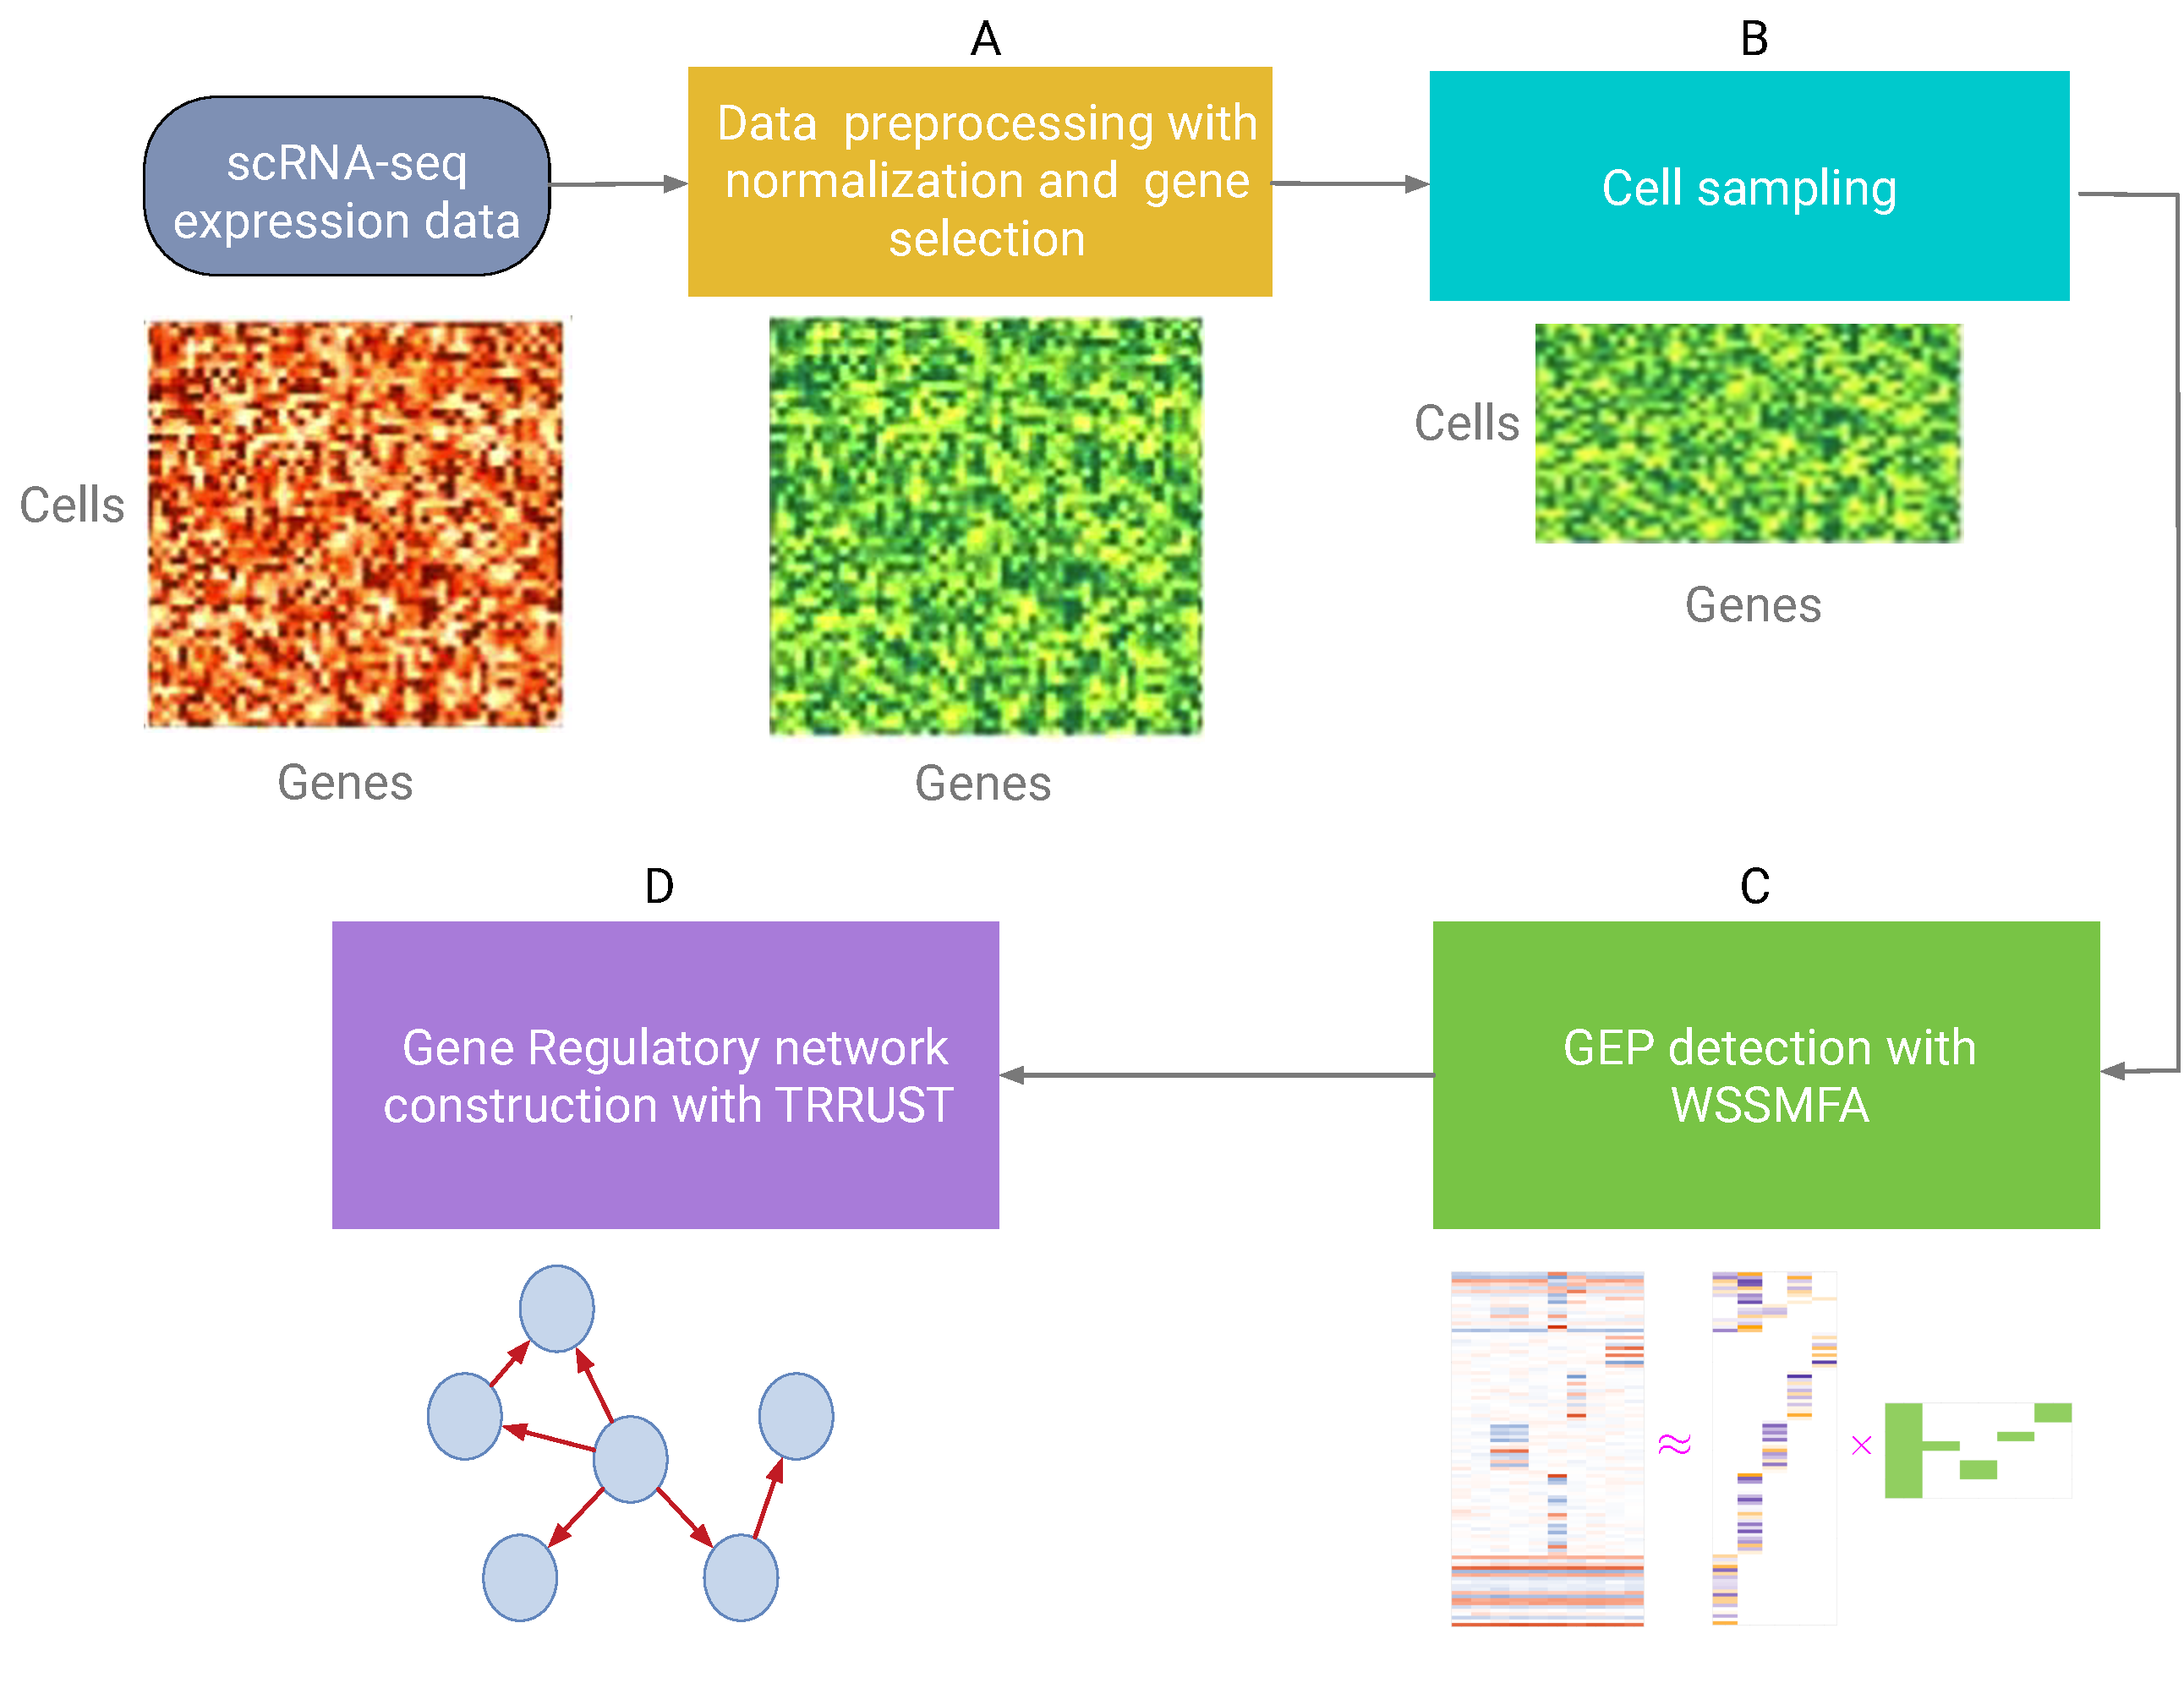
\includegraphics[width=0.8\textwidth]{flowchart-gep.pdf}
    \caption{
        % scGRNHunter flowchart. The input is the scRNA-seq expression data 2D-matrix, whose row stands for cells, column for genes, respectively.
        % (A) Data preprocessing with the input expression data, the output is  a normalized and the column dimension reduced matrix. 
        % Highly expressed genes with a fixed number are chosen for downstream analysis.
        % (B) Cell sampling with a user-defined ratio or a fixed number of cells  from the reduced expression data. 
        % (C) GEP detection with the algorithm WSSMFA. 
        % (D) Gene regulatory network construction with TRRUST.
        scGRNHunter 流程图。
    }
    \label{fig:gep-flowchart}
\end{figure}

\subsubsection{数据预处理}
由于测序技术中的噪声以及基因表达高度稀疏, 因此一般需要对单细胞数据进行预处理来控制数据质量。
通常假定输入的 scRNA-seq 数据是二维矩阵, 行代表细胞, 列代表基因, 矩阵中元素值代表细胞中对应基因的表达量。
对于每个数据集, 本文首先剔除少于 1000 个统一分子标识符 (UMIs) 检测的细胞,
然后过滤掉平均 500 个细胞中累加低于 1 个 count 的基因。
这个过滤后的计数矩阵本文表示为 $X_{ij}$ ($i=1,\ldots,C$ 个细胞, $j=1,\ldots,G$ 个基因)。
然后本文选择由 v-score \upcite{klein2015droplet} 确定的 H 个分散度 (dispersion) 最高的基因作为后续输入。
对于本章中分析的所有数据集上, H 被设置为 500。

在归一化之前选择一个高分散的基因集合是至关重要的, 
因为如果噪声导致的 lower-variance 基因的信号与生物学上有意义的基因信号处在同一个量级上, 那么会对计算不利。 
H 被设置为 500, 主要考虑的是尽量包含足够多的基因保证能检测到微弱的生物信号,同时也要避免包括太多无关的基因使得计算性能欠佳。

\subsubsection{细胞抽样}
类似于 Drop-seq 等技术使得细胞测序规模比较大, 并且本文首先考虑的对象是基因 (即表达矩阵中的列), 
为了加速计算, 可以约定如果待处理的 scRNA-seq 数据上细胞规模大于一个预定的个数, 比如 5000,
本文就可以对矩阵的行 (也就是细胞) 采用行采样。
如果细胞规模个数小于该预定的数值, 直接忽略掉采样这一步, 
直接把所有的细胞纳入到后续计算之中。
 scRNA-seq 数据集下细胞采样的方法除了常见的随机采样外,还有按照细胞类型占比等比例采样 \upcite{sinha2018dropclust},
考虑稀有细胞类型的影响而采用的基于几何学的采样 \upcite{hie2019geometric} 等。

\subsubsection{加权半非负稀疏矩阵分解算法 WSSMFA}

\begin{figure}[!htbp]
    \centering
    \includegraphics[width=0.9\textwidth]{gep_mf.pdf}
    \caption{
        % Illustration of the algorithm WSSMFA.
        % A.Matrix factorization with the scRNA-seq data 2D-matrix. 
        % B.The objective function, where $W$ is the mask matrix, $\alpha$ and $\lambda$ are sparsity penalty parameters, and C is
        % the number of cells.
        算法 WSSMFA 的示意图。
        A. 对 scRNA-seq 数据进行矩阵因子化。
        B. WSSMFA 优化的目标函数,其中 W 为掩码矩阵, $\alpha$ 和 $\lambda$ 为稀疏度惩罚参数, C 为细胞数。
    }
    \label{fig:gep-mf}
\end{figure}

经过上述步骤处理后的 scRNA-seq 数据可以表示为一个矩阵 $X_{C \times G}$, $C$ 为细胞的数目, $G$ 为基因的数目, 
矩阵中的每个值表示该基因在对应的细胞中的表达量。
对于矩阵 $X$, 可以表示为一个因子矩阵 (factor matrix) $F_{G \times K}$ 和一个负荷矩阵 (loading matrix) $L_{C \times K}$,
并且满足 $X=LF^T$, 如图 \ref{fig:gep-mf} A 所示。 

本文设计了一个具有以下三个特征的矩阵分解目标函数:
\begin{enumerate}[label=(\arabic*)]
    \item 对残差加权和的惩罚: 为了考虑基因表达值本身的不确定性,也就是 dropout 效应带来的影响,具有 dropout 值的对应位置处的残差被赋予零权重。
          通过这种方式,基因具有更确定的表达值的对最优参数估计有更大的影响。
    \item 稀疏性: 为了减少过拟合,对分解后的矩阵进行了 $l_1$ 惩罚。
    \item 分解矩阵的半非负性: 因子矩阵捕捉组织间的影响模式,因此,使因子矩阵非负易于解释是一个自然约束。
          同时,由于输入矩阵中数值可能有正有负,因此对负荷矩阵没有这样的约束。
\end{enumerate}
基于此,最终的目标函数定义如下 (如图 \ref{fig:gep-mf} B 所示):
\begin{equation}
    \label{eq:obj}
    \min _{F, L} \frac{1}{2 C}\left\|\left(X-L F^{T}\right) \odot W\right\|_{F}^{2}+\alpha\|L\|_{1}+\lambda\|F\|_{1}
\end{equation}
其中, $F$ 是非负的, $W$ 是 binary 掩码矩阵 (mask matrix), $C$ 是细胞个数,
 $\alpha$ 和 $\lambda$ 是惩罚系数。
$W$ 跟 $X$ 的维度相同,并且有:
\begin{equation}
    W_{i j}=\left\{\begin{array}{ll}1 & \text { if } x_{i j}>0 \\ 0 & \text { otherwise }\end{array}\right.
\end{equation}

这个目标函数是双凸 (biconvex) 的, 也就是说, 只在 $F$ 中凸, 或者只在给定的 $L$ 中凸, 但在两者共同变化时不是凸的。
本文使用交替最小二乘法 (Alternating Least Squares, ALS) 与梯度下降 (gradient descent) 法来优化目标函数 (算法 \ref{alg:wssmfa}, 
在 R 版本 3.5.1 中实现 \upcite{goeman2012penalized,goeman2010l1})。
在每一次迭代中本文固定 F 并更新 L, 然后固定 L 并更新 F, 当两次迭代之间 F 的差值的 Frobenius 范数 < 0.01 时, 更新结束。
在每一步更新中, 优化问题都是有约束条件的线性回归。
由于线性回归的解保证了均方误差与惩罚之和最小,所以代价函数单调下降。
WSSMFA 算法的时间复杂度为 $O(n^2)$, $n$ 为细胞的个数。
\begin{algorithm}
    \renewcommand{\thealgorithm}{5-1}
    \caption{Weighted semi-nonnegative sparse matrix factorization algorithm (WSSMFA)}
    \label{alg:wssmfa}
    \begin{algorithmic}[1]
    \Require  $X_{G \times C}$                                   \Comment{$G$ genes, $C$ cells}
    \Ensure $L_{G \times K}$, $F_{C \times K}$                \Comment{Loading matrix and factor matrix}
        \While{not converged}
            \For{$i = 1 \to G$}                                           
                \State $l_{i} \leftarrow \min _{l_{i}}\left\|\left(x_{i}-l_{i} F^{T}\right) \odot w_{i}\right\|_{F}^{2}+\alpha\left\|l_{i}\right\|_{1}$
                \State which is equivalent to 
                \State $l_{i} \leftarrow \min _{l_{i}}\left\|x_{i} \odot w_{i}-l_{i}\left(F^{T} \operatorname{diag}\left(w_{i}\right)\right)\right\|_{F}^{2}+\alpha\left\|l_{i}\right\|_{1}$
            \EndFor
            \For{$j = 1 \to C$}
                \State $f_{j} \leftarrow \min _{f_{j}}\left\|\left(x_{j}-f_{j} L^{T}\right) \odot w_{j}\right\|_{F}^{2}+\lambda \mid f_{j}\left\|_{1},\right\| f_{j} \| \geq 0$
                \State which is equivalent to 
                \State $f_{j} \leftarrow \min _{f_{j}}\left\|\left(x_{j} \odot w_{j}-f_{j}\left(L^{T} \operatorname{diag}\left(w_{j}\right)\right)\right)\right\|_{F}^{2}+\lambda\left\|f_{j}\right\|_{1},\left\|f_{j}\right\| \geq 0$
            \EndFor
        \EndWhile  
        \State \Return $L$, $F$        
  \end{algorithmic}
\end{algorithm}

\subsubsection{构建单细胞 GRN}

针对因子矩阵 (factor matrix) $F_{G \times K}$, 每一个因子代表了一个 GEP, 
身份 GEPs 里面的基因没有交集, 活动 GEPs 跟各个身份 GEP 之间一般存在相交的基因, 
针对身份 GEP 和活动 GEP 本文根据基因列表可以在 TRRUST 线上服务上查询关键的调控因子 (Transcription Factor, TF),
然后构建基因调控网络。


%根据 GEP 结合 TRRUST 数据库找到 TF, 然后构建得到整个的基因调控网络。

TRRUST (version 2, \upcite{han2018trrust}) 是一个采用数据挖掘技术辅助建立的人类和小鼠转录调控网络数据库,
该数据库还提供了网页版本的服务。
当前版本的 TRRUST 分别包含 800 个人类 TFs 和 828 个小鼠 TFs 的 8,444 和 6,552 个 TF-target 调控关系对。
TRRUST 数据库还提供了调控模式的信息 (激活或抑制)。
目前已知调控模式的调控关系有 8972 个 (59.8\%)。

\subsection{实验结果}
\subsubsection{数据集}
本章中实验使用的数据集如表 \ref{tab:dataset} 所示。
需要注意的是, 聚类的结果和原始的 count 矩阵在 GEO 中无法获取到,
因而从文献的作者那里获得了聚类的标签和非规范化的原始数据。
原始的 scRNA-seq 数据中一共包含 66889 个细胞, 每个细胞包含 25984 个基因。
文献作者提供的细胞标签总计包含 10 个类别 C1、C2、\ldots、C10, 
其中 C4 和 C5 分别还包括 5  和 6 个子类别, 详细的类别列表如下:
`C1 - Meso. Precursors', 
`C2 - Astroglia', `C3 - Dop. Neurons', 
`C4 - Forebrain',
`C4 - Forebrain - Callosal neurons',
`C4 - Forebrain - Corticofugal neurons',
`C4 - Forebrain - Intermediate progenitors',
`C4 - Forebrain - Interneurons',
`C4 - Forebrain - Radial glial cells', 
`C5 - Retina',
`C5 - Retina - Amacrine cells', 
`C5 - Retina - Bipolar cells',
`C5 - Retina - Mueller glia', 
`C5 - Retina - Photoreceptors',
`C5 - Retina - Pigmented epithelia',
`C5 - Retina - Retinal ganglion cells', 
`C6', `C7', `C8',
`C9 - Neuroepi. cells',
`C10 - Prol. precursors'。

\begin{table}[!htbp]
    \caption{使用的公开数据集描述} 
    \label{tab:dataset}
    \resizebox{\columnwidth}{!}{%  
    \begin{tabular}{lllll}
    \hline
    Author(s)                           & Year & Dataset title                                                                                                              & Dataset URL                                                                                               & Database and Identifier                                                                          \\ \hline
    \multicolumn{1}{c}{Quadrato G, et.} & 2017 & \begin{tabular}[c]{@{}l@{}}Cell diversity and network \\ dynamics in photosensitive \\ human brain organoids.\end{tabular} & \begin{tabular}[c]{@{}l@{}}https://www.ncbi.nlm.nih.gov\\ /geo/query/acc.cgi?\\ acc=GSE86153\end{tabular} & \multicolumn{1}{c}{\begin{tabular}[c]{@{}c@{}}Gene Expression Omnibus, \\ GSE86153\end{tabular}} \\
    \hline    
    \end{tabular}
    }
\end{table}

\subsubsection{参数设置}
WSSMFA 算法的超参数,包括因子个数 ($K$) 和稀疏惩罚参数 ($\alpha$,$\lambda$)。
本文在 [20,25,30,35,40] 范围内评估 $K$, 在 [4.9,24.5,49,245,490] 范围内评估 $\alpha$ 和 $\lambda$。
这些范围的选择是通过考虑单细胞中的一些已知的先验知识比如类别数来定义 $K$ 的可信值,
并通过手动检查 $\alpha$ 和 $\lambda$ 变化很大的范围,
以避免对这些超参数的范围进行高分辨率搜索,导致明显不合理的解,
如因子缺乏稀疏性或者大量为空,或者与原始数据间没有关联性。

在指定的搜索空间内,利用之前定义的矩阵分解稳定性标准和学习因子的独立性,即代表足够的稀疏性,
本文对所有 $K$、$\alpha$ 和 $\lambda$ 组合的模型进行了评估。
考虑到矩阵因子化的随机性, Brunet 等人 \upcite{brunet2004metagenes,wu2016stability} 提出了一种寻找最稳定的因子化结果的方法,
这种方法已经在各种研究中得到应用。
本文对每个模型进行随机初始化,运行 30 次后得到共识矩阵 $C$。
$C$ 中的值在 $0$ 和 $1$ 之间,代表一对细胞被分配到同一个因子的比例。
本文随后利用 $C$ 矩阵,计算了共识相关性,用于衡量 $C$ 矩阵的离散程度。
共识相关度越高,说明因子矩阵越稳定。

对于每一个观察到的学习到的非空因子 $K^\textup{'}$ 的平均数 (可能小于输入的 $K$),
对 $\lambda$ 和 $\alpha$ 的不同取值进行了汇总,
本文计算了中位共线性相关性 (cophenetic correlation,\upcite{brunet2004metagenes}),
剔除了任何对应于 K 的中位共识相关性 $< 0.9$ 的 $K^\textup{'}$。
接下来,在剩下的单个设置中,排除任何一个共线性相关性 $< 0.9$ 的参数取值。
最后,在这些明显稳定的设置中,根据因子对之间的最小皮尔逊相关性选择最终的超参数,
使得独立的因子和与数据中独立信号的稀疏程度相匹配。
在这里,计算了每对因子的皮尔逊相关性,计算一对相关矩阵的 Frobenius 范数, 
并在 30 次相同设置的随机初始化运行中取平均值。

\subsubsection{实验结果分析}
%\subsubsection{WSSMFA 揭示了基因表达程序的存在}

在大脑类器官数据集上,在数据预处理之后保留了 500 个分散度最高的基因 ($H = 500$),
按照 0.05\% 的比例随机采样,抽取了 2623 个细胞。
抽样后的 scRNA-seq 数据使用基于 t 分布的随机邻域嵌入 (t-SNE) 方法并结合已知的细胞的类别标注信息进行可视化。
需要注意的是细胞类别标签来自于用户输入,
或者是采用第 \ref{sec:rafclust} 章提出的 RafClust 方法或是 Seurat Clustering 等方法获取细胞类别的差异表达基因后手动注释的细胞类别标签, 
WSSMFA 算法本身是不需要细胞类别标签的但是在后续 GRN 构建和分析的时候需要用户提供细胞类别标签信息。
t-SNE 图来反应了 scRNA-seq 数据中细胞分布的宏观结构,
可以看出 scRNA-seq 数据是否有不同的类别,
即细胞是否存在异质性,
对大脑类器官数据集的可视化结果如图 \ref{fig:gep-tsne} 所示。
按照模型选择的步骤操作后,
最终确定参数设置为: $K = 15$, $\alpha = 50$, $\lambda = 5$, 
即 15 个因子 (f1, f2, $\ldots$, f15),也就是对应 15 个 GEP。
负荷矩阵 $L$ 揭示了各细胞的表达量与因子之间的组合线性关系,本文按照细胞类别对负荷矩阵进行统计,
针对每个 GEP 可以画出对应类别的负荷的箱形图 (boxplot),如图 \ref{fig:gep-gep} 所示。
将 GEP1,GEP2,\ldots,GEP15 和图 \ref{fig:gep-tsne} 叠加起来可视化,
用以观察各个 GEP 在该 scRNA-seq 数据中各个细胞类别中的分布,
结果如图 \ref{fig:gep-distribution} 所示。

\begin{figure}[!htbp]
    \centering
    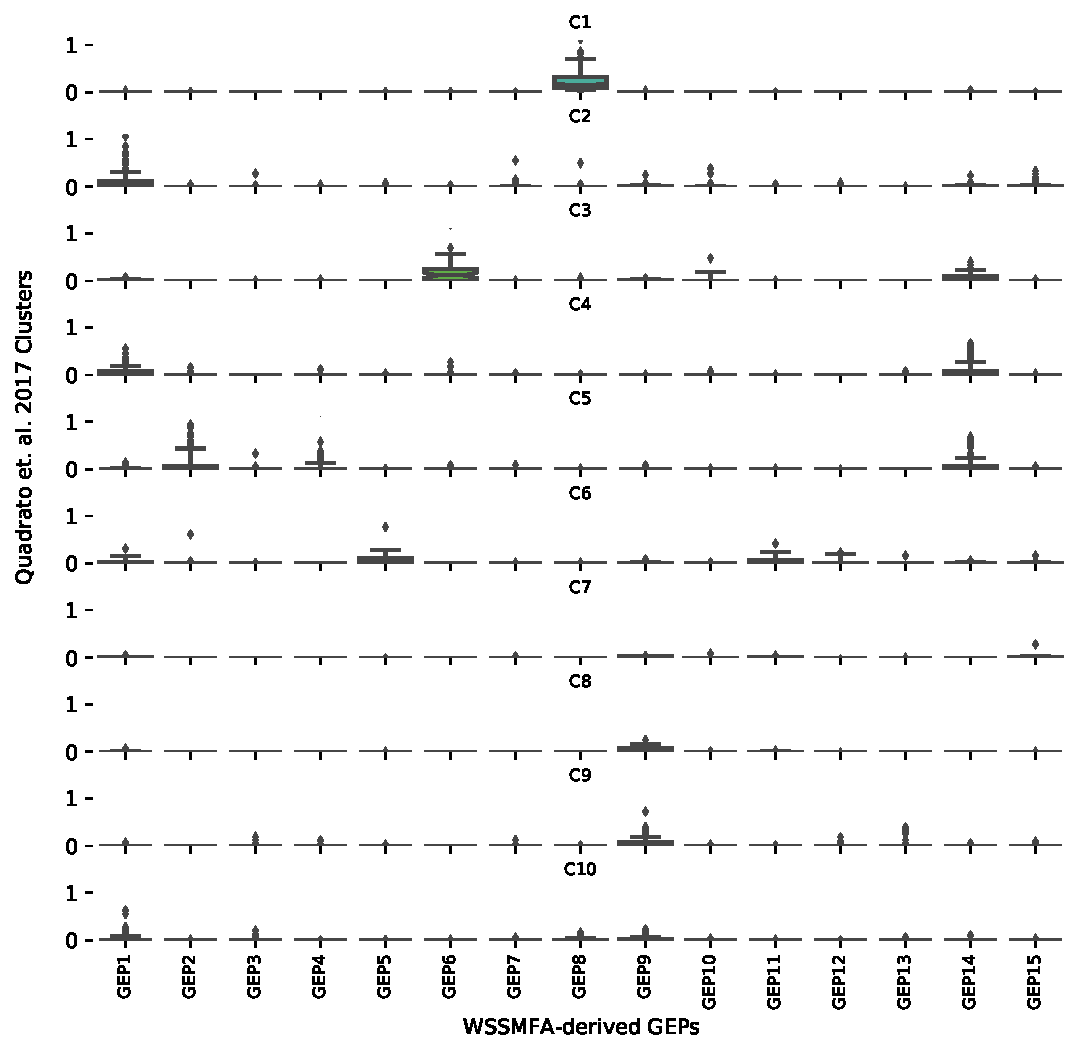
\includegraphics[width=0.9\textwidth]{GEP_Usage_Vs_Published_Clusters_QuadratoEtAI.pdf}
    \caption{
    % GEPs detected with WSSMFA.
    % GEP1, GEP2, $\ldots$, GEP15 are the 15 GEPs derived with WSSMFA algorithm.
    % For each GEP, the loading values based on the 10 different clusters,i.e. C1, C2, $\ldots$, C10,  
    % are visualized with boxplot.
    算法 WSSMFA 检测到的 GEPs 示意图。
    }
    \label{fig:gep-gep}
\end{figure}

\begin{figure}[!htbp]
    \centering
    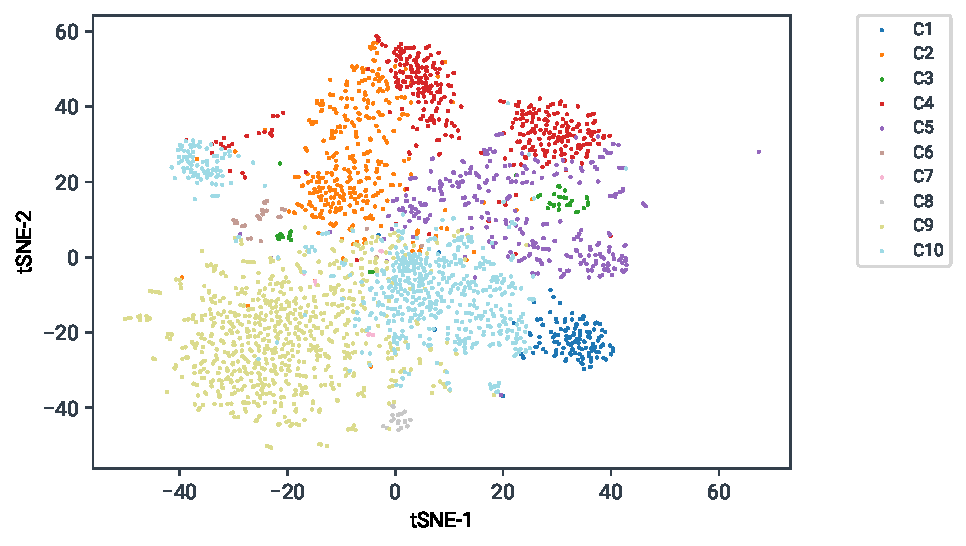
\includegraphics[width=0.9\textwidth]{GEP_tsne_2d_QuadratoEtAI.pdf}
    \caption{
    %The sampled brain organisms data visualized with t-SNE.
    采样后的大脑器官数据使用 t-SNE 及细胞类别标签进行可视化。
    }
    \label{fig:gep-tsne}
\end{figure}

\begin{figure}[!htbp]
    \centering
    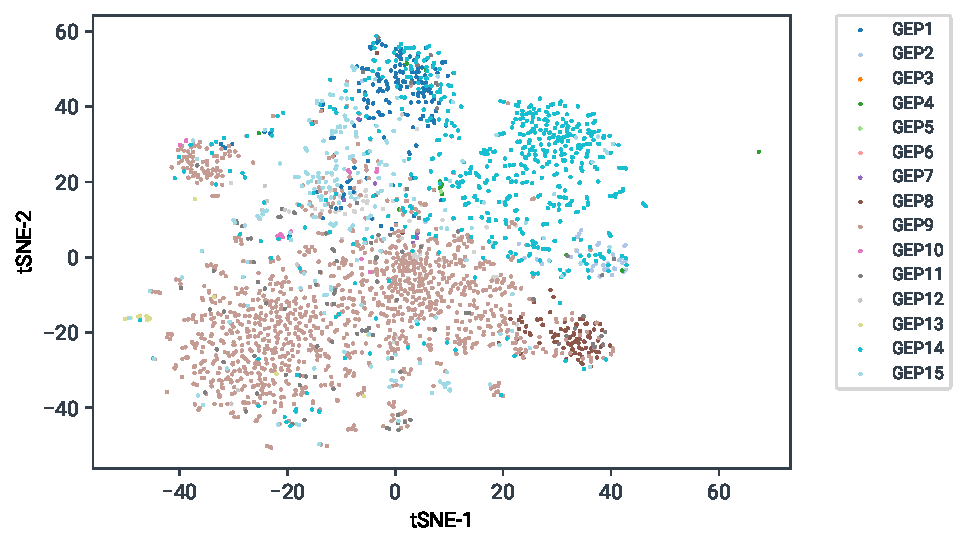
\includegraphics[width=0.9\textwidth]{GEP_tsne_2d_loading_QuadratoEtAI.pdf}
    \caption{
    %The sampled brain organisms data visualized with t-SNE.
    采样后的大脑器官数据上所有的 GEPs 分布可视化。
    }
    \label{fig:gep-distribution}
\end{figure}

\begin{figure}[!htbp]
    \centering
    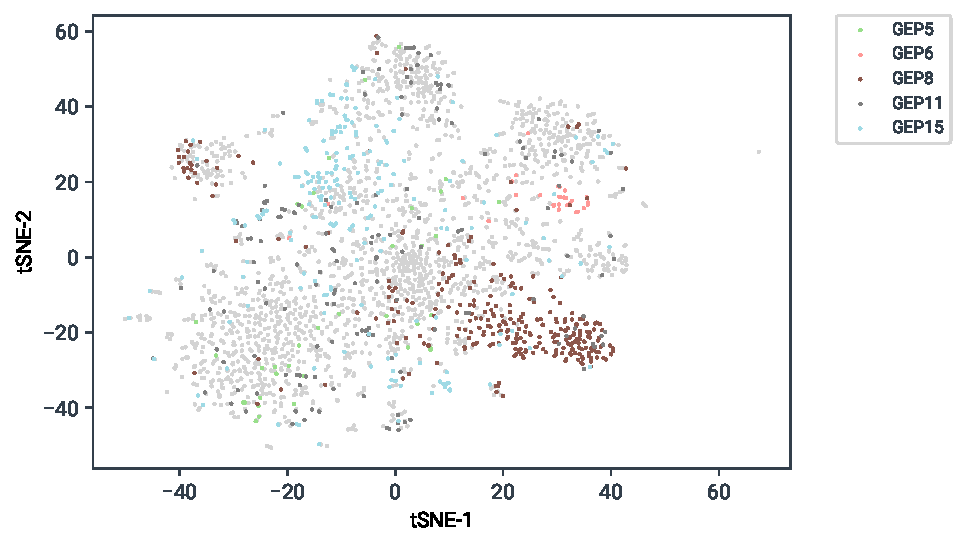
\includegraphics[width=0.9\textwidth]{GEP_tsne_2d_identitygep_QuadratoEtAI.pdf}
    \caption{
    %The sampled brain organisms data visualized with t-SNE.
    大脑器官数据上的身份 GEPs 分布可视化。
    }
    \label{fig:gep-identitytsne}
\end{figure}

\begin{figure}[!htbp]
    \centering
    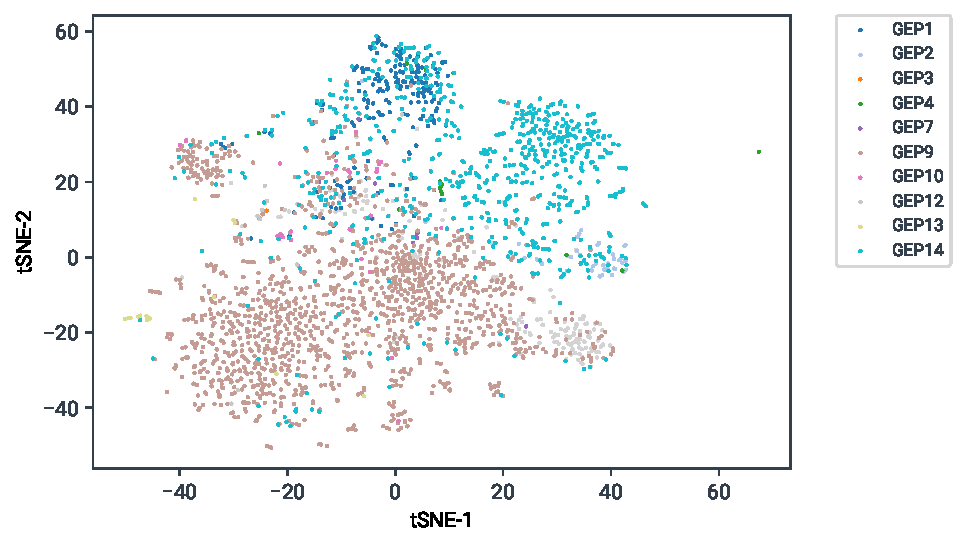
\includegraphics[width=0.9\textwidth]{GEP_tsne_2d_activegep_QuadratoEtAI.pdf}
    \caption{
    %The sampled brain organisms data visualized with t-SNE.
    大脑器官数据上的活动 GEPs 分布可视化。
    }
    \label{fig:gep-activetsne}
\end{figure}

如果结合单细胞数据集的细胞类别标签,可以判断 GEP 是不是身份 GEP 或者是活动 GEP。
如果一个 GEP 仅仅在一个细胞类别中表达, 那么它就是一个身份 GEP;
如果在两个或者多个细胞类别中表达,那么它就属于活动 GEP。
结合图 \ref{fig:gep-gep}、图 \ref{fig:gep-tsne} 和图 \ref{fig:gep-distribution} 可以看出, 
GEP6 和 GEP8 是典型的身份 GEPs (分别对应到类别 C3 和 C1), GEP1、GEP9 和 GEP14 是典型的活动 GEPs。
GEP1 牵涉到类别 C2、C4、C6 和 C10; GEP14 牵涉到类别 C3、C4 和 C5。
身份 GEPs 如图 \ref{fig:gep-identitytsne} 所示,
活动 GEPs 如图 \ref{fig:gep-activetsne} 所示。

%\subsubsection{身份调控网络与活动调控网络的构建}

结合因子矩阵 $F$,每一列中系数不为零的基因即是该因子 (也就是 GEP) 中所包含的基因,
针对每个 GEP,可以结合 TRRUST (version 2) 提供的 web service 获取这些基因的 TF 从而构建其 GRN。
显然,基于单细胞上的聚类分析和差异表达基因分析的方法只能构建身份GRN, 无法构建活动 GRN。
差异表达基因分析后,每个类别的marker 基因集合获取到之后, 
然后利用 TRRUST 找到对应的 TF 转录因子后构建身份 GRN。
STRING (https://string-db.org/) 蛋白质相互作用数据库,
是 Search Tool for the Retrieval of Interaction Gene/Proteins 的缩写,
该数据库中收录了已知和预测的蛋白质/基因间的相互作用关系,比较完整。
本文利用 STRING 提供的人类 GRN 数据集作为 GRN 构建的金标准网络来评测相关方法的性能, 
该网络数据集总共包含 198285 条已确认的基因调控关系。

为了测试 scGRNHunter 在构建单细胞身份 GRN 上的效果,
本文选择了在单细胞上差异表达基因分析构建身份 GRN 与之进行对比。 
利用 Seurat 这个流行的单细胞数据分析软件 R 包对该数据集进行分析,
由于该数据集已经提供了细胞类别标签,因此不使用 Seurat 的聚类方法。
每一个类别的细胞的差异表达基因是利用 Seurat 提供的 FindAllMarkers 函数获取, 
差异表达分析时候默认采用的是 Wilcoxon Rank Sum Test。
从细胞类型的角度来看, 
C1 这个细胞类型对应的是身份 GEP,也就是 GEP8, 如图 \ref{fig:gep-tsne} 所示。
首先对比 C1 类别的差异表达基因和利用 WSSMFA 算法获取的 GEP8 的基因, 如图 \ref{fig:gep-grn-comparison} A 所示。
Seurat 的差异表达基因 和 WSSMFA 算法得到的基因在 C1 细胞类别上重合率为 14\%, 且前面的差异表达得到的基因数目偏多。 
利用 C1 类别的差异表达基因结合 TRRUST 数据库查找每个目标基因的转录因子后, 
将得到的 GRN (如图 \ref{fig:gep-grn-comparison} B 左图所示)和利用 scGRNHunter 方法得到的 GRN (如图 \ref{fig:gep-grn-comparison} B 右图所示)
分别计算其 GRN 的准确率 accuracy。
在图 \ref{fig:gep-grn-comparison} B 所示的两个网络中, TF 是用蓝色节点来表示, TG 则是用红色节点表示。
如图 \ref{fig:gep-grn-comparison} C 所示, 对比方法构建的 GRN 准确性只有 0.29, 
而利用 scGRNHunter 构建的 GRN 准确性达到了 0.39, 从准确率上 scGRNHunter 提高了 34\%。
该实验表明, scGRNHunter 能够构建准确的单细胞身份 GRN。

\begin{figure}[!htbp]
    \centering
    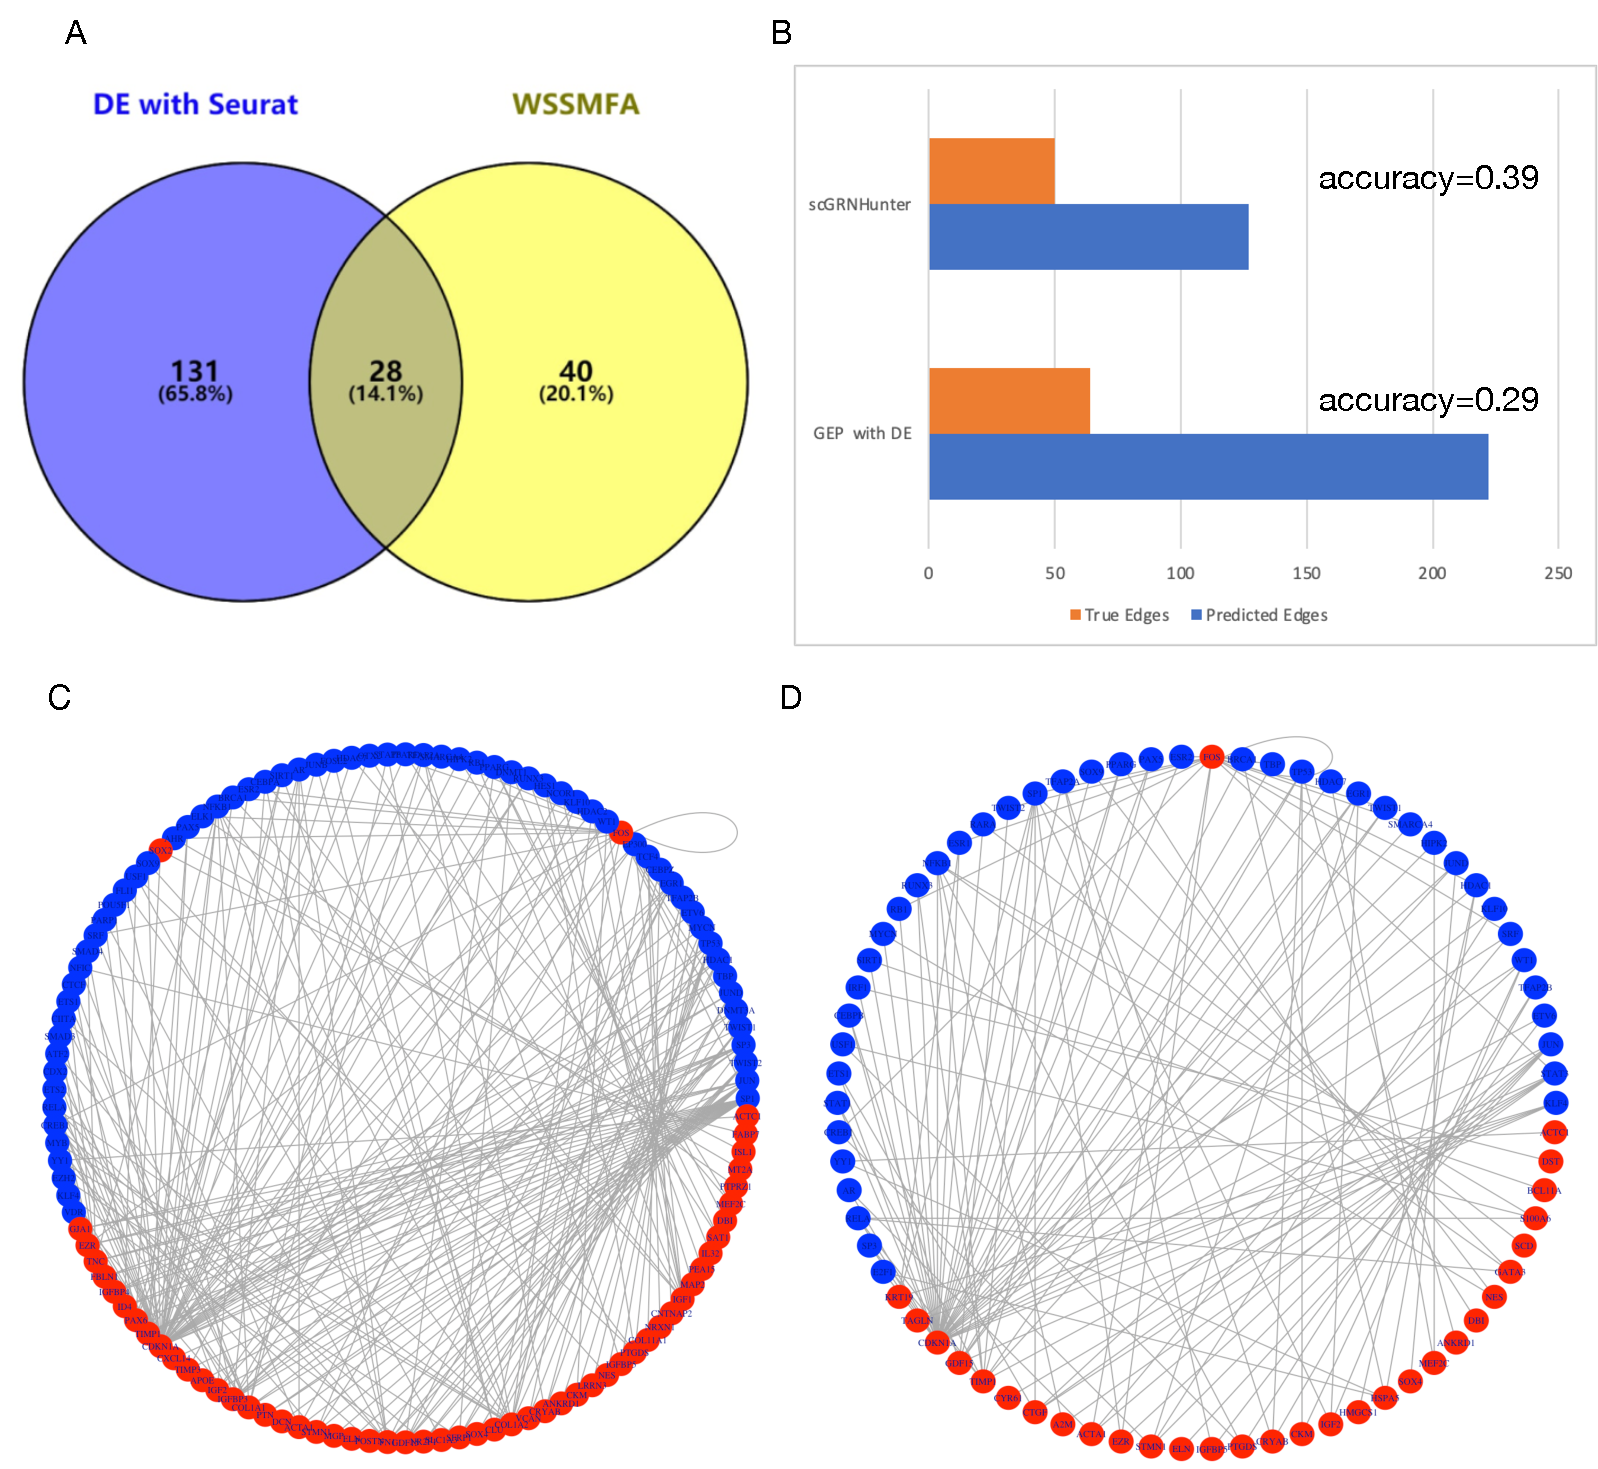
\includegraphics[width=1\textwidth]{gep_analysis.pdf}
    \caption{细胞类别 C1 的身份 GRN 构建结果对比示意图。}
    \label{fig:gep-grn-comparison}
\end{figure}

% \begin{figure}[!htbp]
%     \centering
%     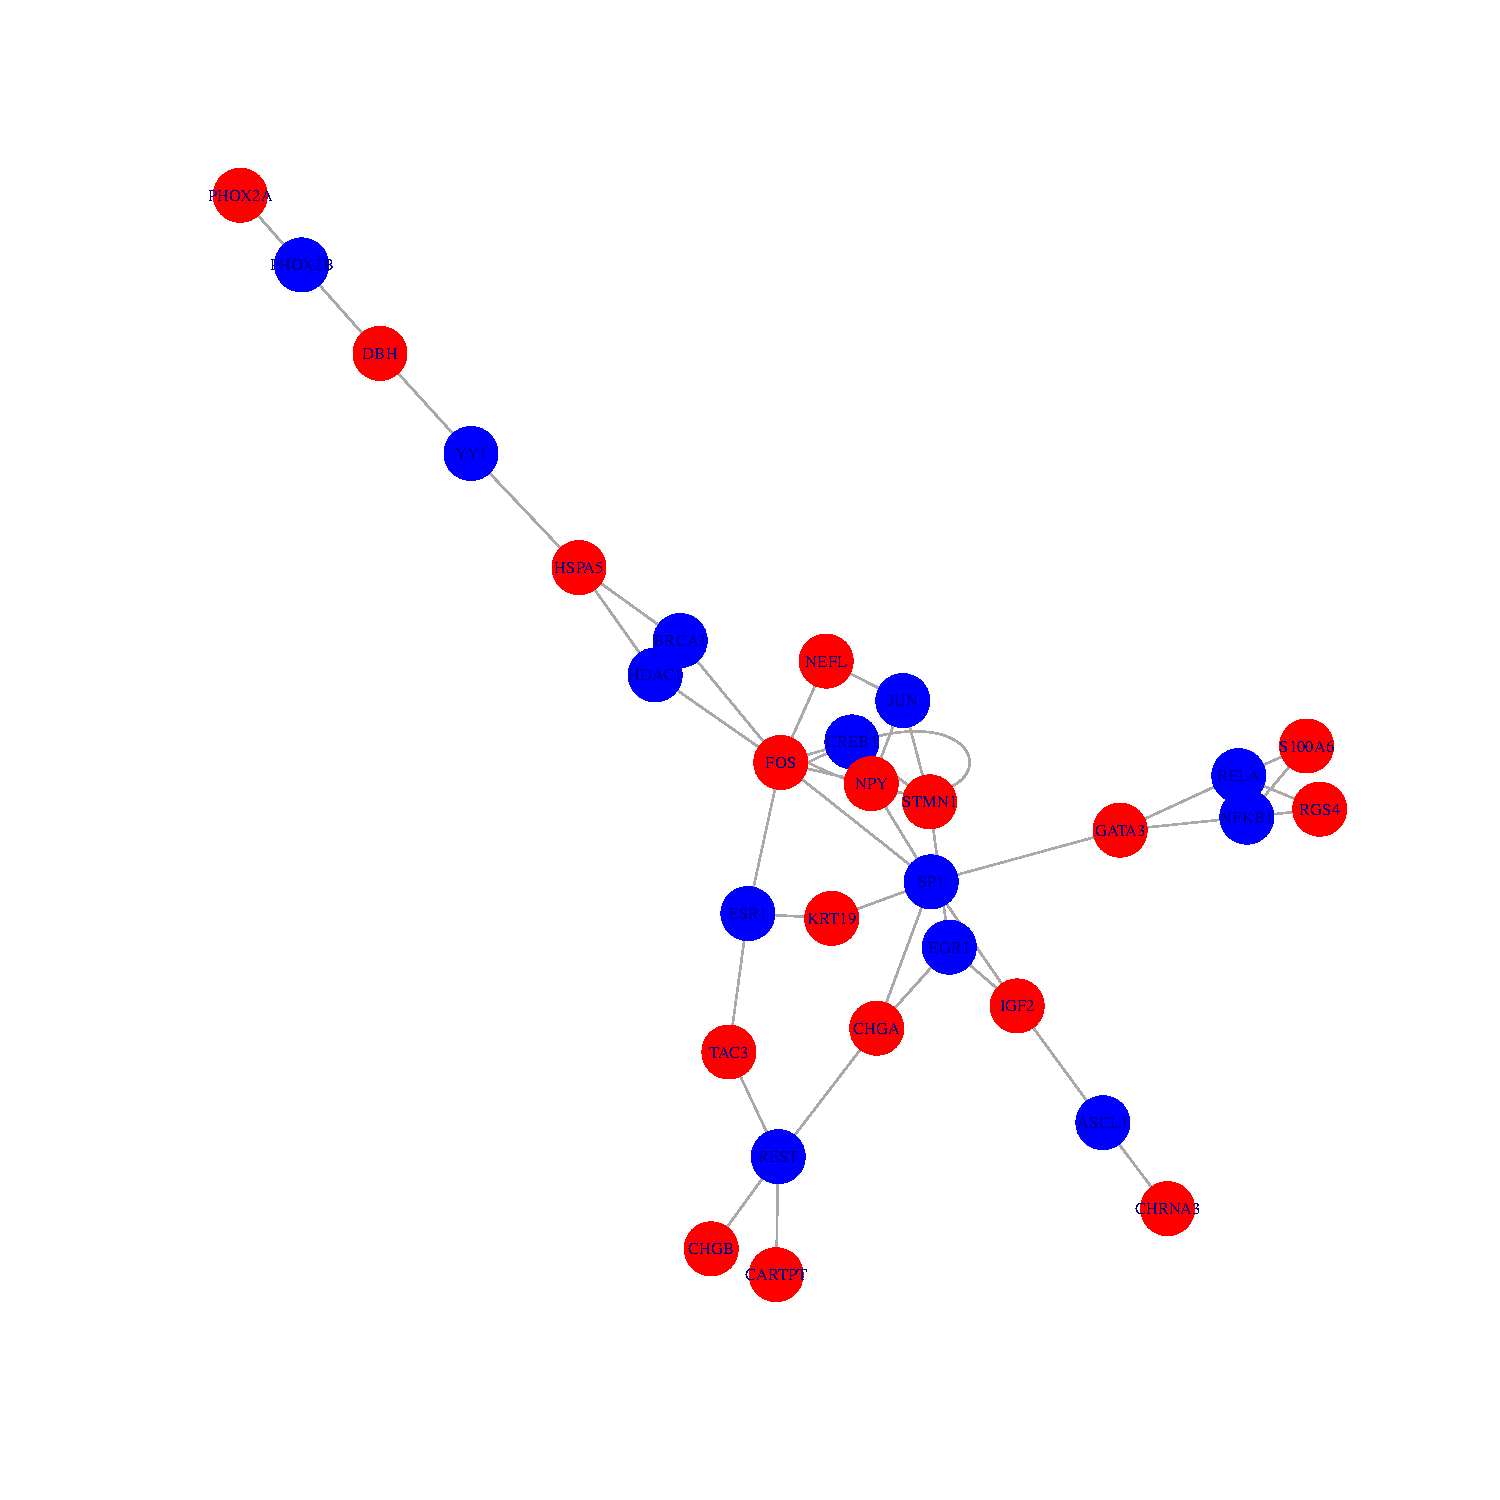
\includegraphics[width=1\textwidth]{GEP6.pdf}
%     \caption{由 GEP6 构建的基因调控网络。}
%     \label{fig:gep-grn-gep6}
% \end{figure}

目前还没有文献提出构建单细胞活动 GRN, 
scGRNHunter 是所知的构建单细胞活动 GRN 的第一个方法。
结合图 \ref{fig:gep-gep} 、图 \ref{fig:gep-tsne} 可知, 
GEP14 是对应到细胞类别 C4、C5、C6 的活动 GEP。
对 GEP14 进行 GO (Gene Ontology, 基因本体) 富集分析, 发掘基因集合在 BP 生物过程上的功能, 如图 \ref{fig:gep-active} A 所示。
该 GEP 主要与神经发育的相关活动过程相关, 且有着统计学上的显著性。
由 GEP14 构建的单细胞活动 GRN 如图 \ref{fig:gep-active} B 所示, 包含 122 个节点, 195 条调控边。
该实验表明, scGRNHunter 对于构建单细胞活动 GRN 具有一定的参考意义。

\begin{figure}[!htbp]
    \centering
    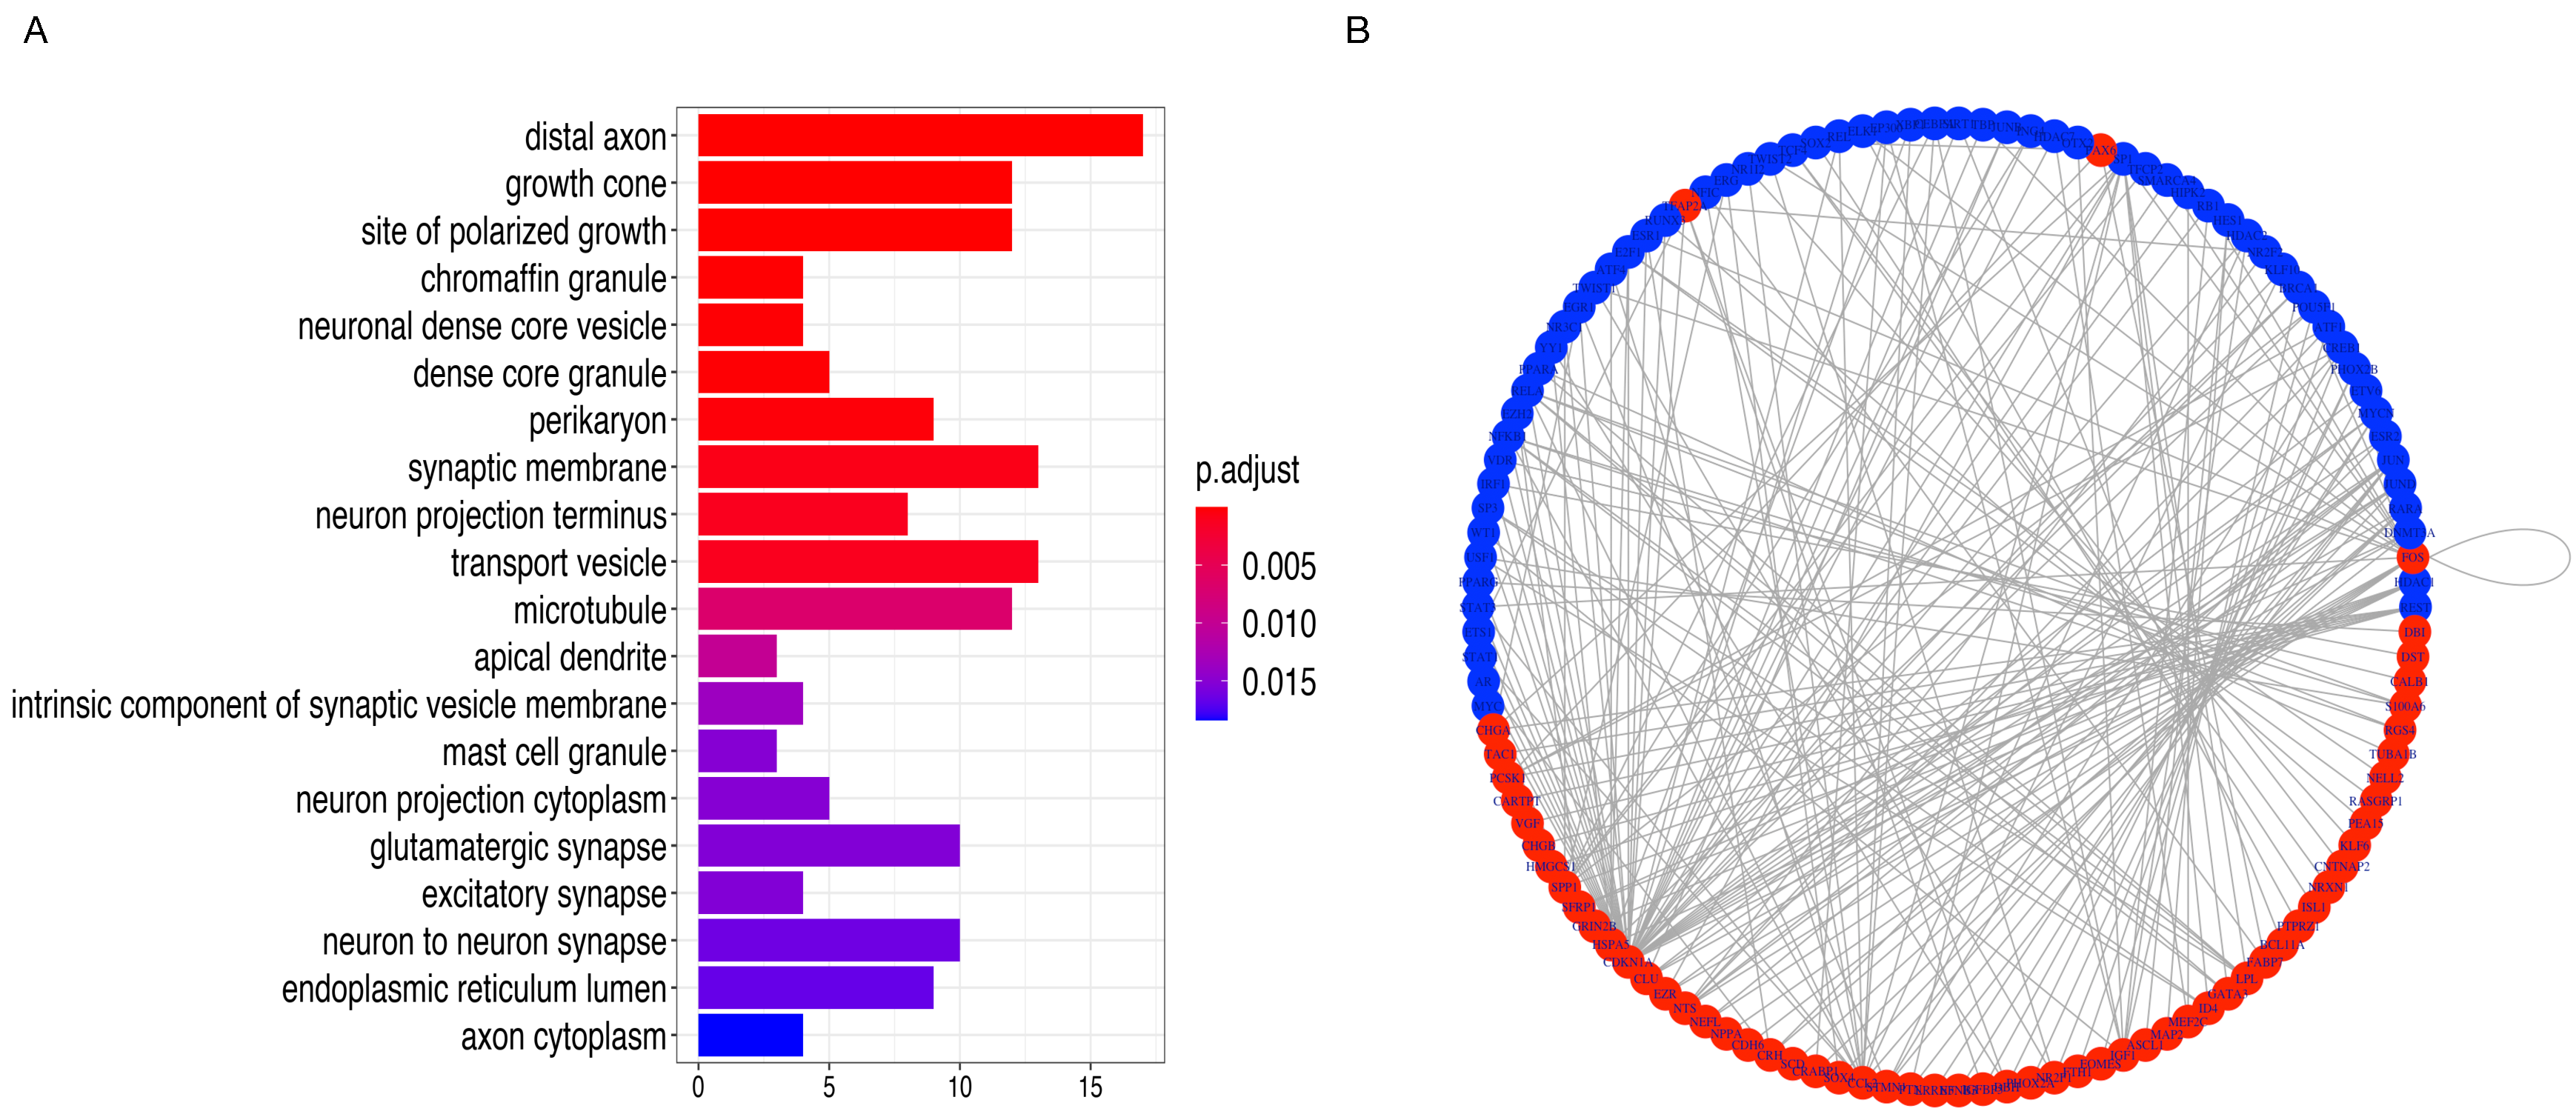
\includegraphics[width=1\textwidth]{gep_active.pdf}
    \caption{由 GEP14 构建的单细胞活动 GRN 及其富集性分析。}
    \label{fig:gep-active}
\end{figure}


% 由 GEP6 构建的基因调控网络如图 \ref{fig:gep-grn-gep6} 所示,
% 该网络总共包含 30 个节点 (TF 用蓝色节点表示, TG 用红色节点表示,下同), 41 条调控边。默认的调控方向都是 TF 调控 TG, 因此在基因调控网络的可视化图中本文不显式突出边的方向。

% \begin{figure}[!htbp]
%     \centering
%     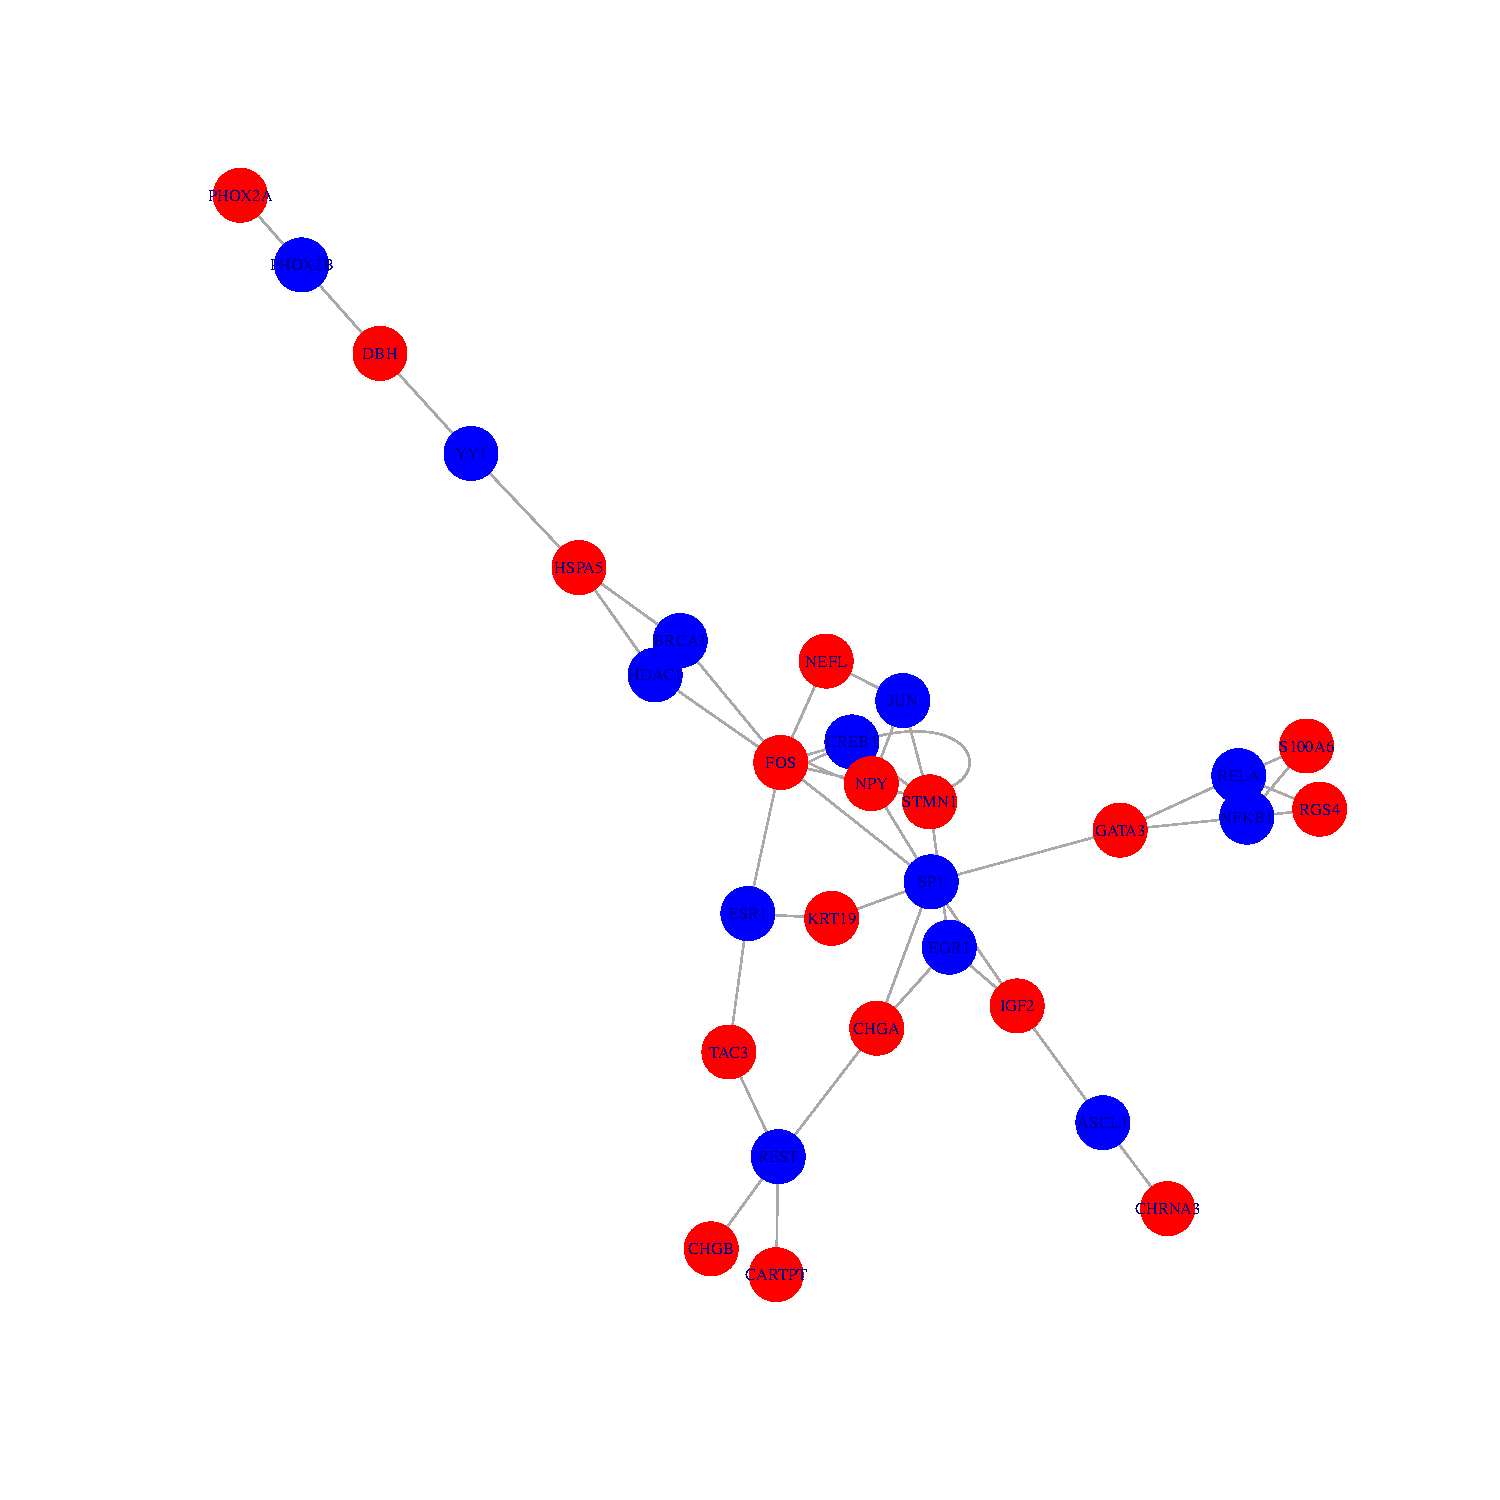
\includegraphics[width=1\textwidth]{GEP6.pdf}
%     \caption{由 GEP6 构建的基因调控网络。}
%     \label{fig:gep-grn-gep6}
% \end{figure}


% 由 GEP14 构建的基因调控网络如图 \ref{fig:gep-grn-gep14} 所示。
% 该网络总共包含 122 个节点, 195 条调控边。
% \begin{figure}[!htbp]
%     \centering
%     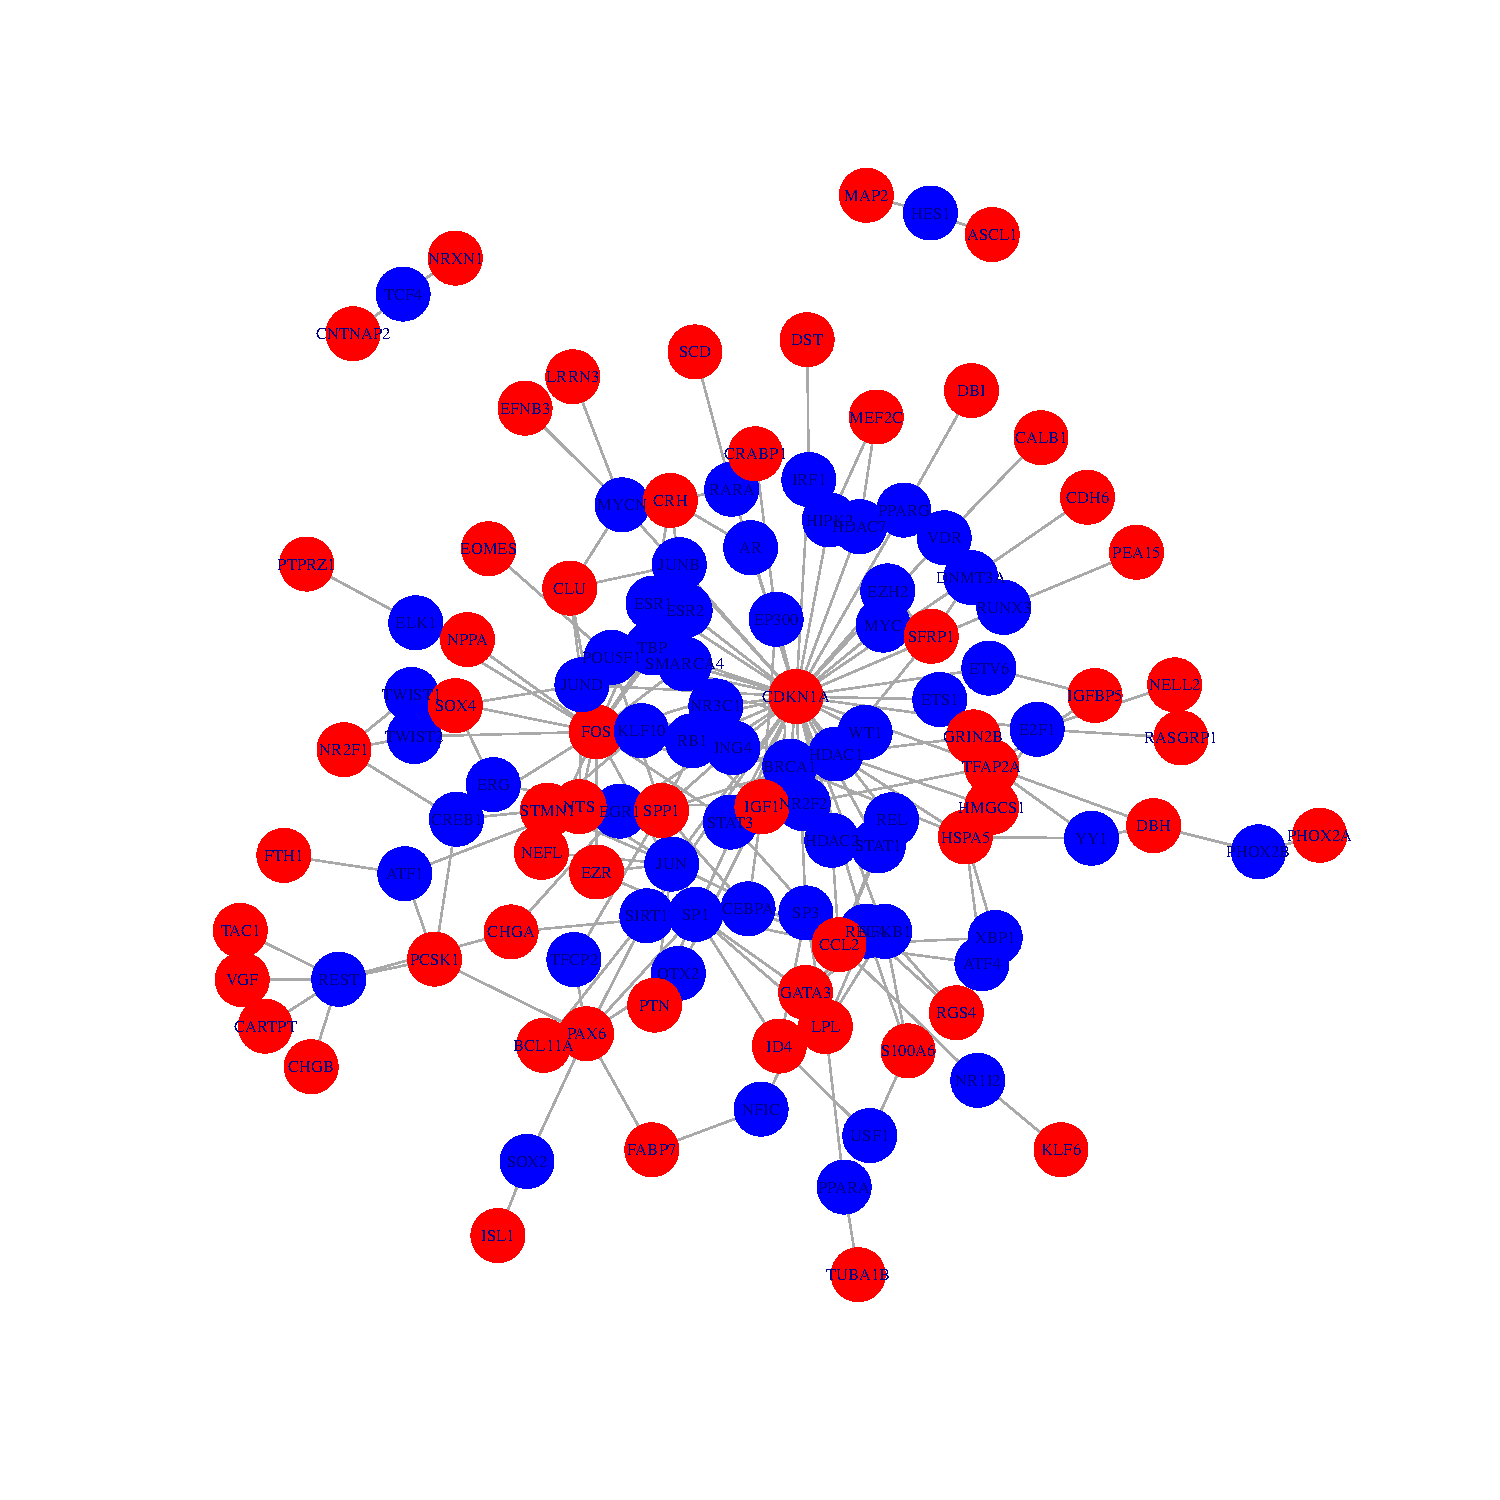
\includegraphics[width=1\textwidth]{GEP14.pdf}
%     \caption{由 GEP14 构建的基因调控网络。}
%     \label{fig:gep-grn-gep14}
% \end{figure}


\subsection{小结}
scGRNHunter 的核心算法依赖 WSSMFA 矩阵分解算法,
该方法的前提假设是细胞的表达可以被建模为 GEPs 的线性组合,
这也是该方法的一个限制。
值得注意的是, 这排除了转录抑制的建模, 也就是说其中一个或多个基因将被一个 GEP 诱导,
当第二个抑制 GEP 在同一细胞中活跃时, 其表达量会显著降低。
据本文所知, 这种关系还没有在矩阵因子化框架中表示, 但它们可能更容易纳入新的潜变量模型类别,
如变分自动编码器 (Variational Auto-encoders, VAEs) \upcite{ding2018interpretable,gronbech2018scvae}。
VAEs 代表了一个高度灵活的隐式空间中的建模, 可以捕捉隐式变量之间的非线性和相互作用。
然而, 虽然隐变量的设计是为了促进输入基因表达数据的准确重建, 
但它们是否可以直接或间接地解释为不同的 GEPs 相互作用, 还有待证明。
在可预见的未来, 调控关系的建模需要综合权衡考虑模型本身的灵活性与训练和解释它们的输出的难度这两个方面。

随着 RNA 捕获效率和高通量的技术不断地进步, scRNA-seq 数据可能会变得更加丰富和精准,
这将使得检测越来越细微的 GEPs, 从而捕捉细胞类型、细胞状态和活动的生物变异性,而不需要进行实验操作成为了可能。
本章提出了一个计算方法框架 scGRNHunter,
该方法使用了基于矩阵分解的算法 WSSMFA 直接从 scRNA-seq 中构建出这样的 GEPs。 
通过在公开的大脑类器官 scRNA-seq 数据集上的实验表明,
本章提出的 scGRNHunter 方法可以准确地构建出身份和活动性的子程序, 
并在此基础上构建成基于细胞类别身份的基因调控网络和基于细胞活动的基因调控网络。
scGRNHunter 为细胞和组织行为提供了至关重要的解释角度,
为基于 scRNA-seq 数据的基因调控网络的构建提供了一个全新的思路。
后续我们将结合该计算方法, 进一步寻找生物上的实验结果支撑。